\section{The complete collection of interfaces}\label{loop:section}

We identify every macroscopic interface, including its traversal order
and its place in the nested collection.  Write $H_n:X_n\to\Chat$
for the homeomorphisms of the
topological correspondence and $\eta:[0,1]\to\Chat$ for the limiting
space-filling exploration, in the common coupling with the surface and
all retained observations.  In particular, $\eta(0)=\eta(1)=p_*$,
the images under $H_n$ of the flag triangles have maximum diameter tending
to zero, and the spatial representatives of the discrete tour converge
uniformly to $\eta$.  All the results of this section concern that
correspondence; the final coordinate change is made in
Proposition~\ref{loop:canonical}.

There are two steps.  Exact surgery on the finite exploration tour
represents each FK loop by a face of a noncrossing chord system.
Convergence of all these faces gives a complete collection of ordered
limiting curves, with no extra macroscopic loops.  We then identify
these curves with CLE.  Exploration switches first identify each curve
as a closed initial portion of a CLE traversal; a two-sided winding
test rules out any nonconstant omitted portion.

The loop readout follows Sheffield's exploration-tree construction of
CLE \cite{SheffieldExplorationTrees} and its realization through
imaginary-geometry flow and counterflow lines \cite{MillerSheffieldIGIV}.
The alternating nested exploration is also used in
\cite[Section~2.1.6]{AruHoldenPowellSunCritical}. Finite-volume contour and
cone-time convergence comes from \citet{GwynneSunFKIII}; the argument
here upgrades it to simultaneous ordered-curve convergence in the
canonical conformal embedding.

\subsection{Flexible orders as a closed chord system}

Let $\mathbb T=\R/\Z$, identified with the boundary of the closed unit disk
$\overline{\mathbb D}$ by $t\mapsto e^{2\pi it}$.  For $a,b\in\mathbb T$,
write $[a,b]_{\rm d}$ for the straight chord joining their images.  This
notation distinguishes a disk chord from an interval in exploration time.
A \emph{chord system} is a closed set of unordered endpoint pairs, including
all diagonal pairs.  Its underlying lamination is the union of its chords
and $\partial\mathbb D$.  Noncrossing means that two distinct chords have
disjoint relative interiors.  A \emph{face} is a connected component of the
complement of the lamination in $\mathbb D$; faces are open convex sets.

For the length-$2n$ word, fix the distinct occurrence times
\[
 t_k=\frac{k-1/2}{2n},\qquad 1\le k\le2n.
\]
Here $t_k$ labels the visit in the interior of the $k$th step of the
abstract medial tour.  It does not assert an exact scalar-chord identity
at the interpolated contour height.  For a flexible order at position
$j$, with matched burger at $i<j$, use the chord $[t_i,t_j]_{\rm d}$,
labelled by that burger's type.  Adjoin the diagonal pairs to obtain
$\mathcal E_n$.  Every letter belongs to at most one flexible pair,
so these chords have distinct endpoints, even for consecutive matched
letters.  This convention is needed for the exact face surgery below.
The adjacent-cut times used in the contour limit differ by at most
$1/(2n)$; their replacement by $t_i,t_j$ preserves all limiting
endpoint assertions.  Spatial tracking at these occurrence times
follows from tracking at adjacent cuts, continuity of $\eta$, and
the vanishing image diameter of the intervening flags.

For the limiting excursion $Z=(L,R)$, a backward cone interval is
\[
 [v(t),t],\qquad
 v(t)=\inf\{s<t:L(u)\ge L(t),\ R(u)\ge R(t)
                         \text{ for }u\in[s,t]\}.
\]
Here $t$ is required to admit at least one such interval of positive
length.  Away from the end convention, precisely one coordinate agrees
at its two endpoints; this coordinate labels the entrance wall.  We use
the corresponding burger-type label.  Let $\mathcal E$ consist of the
circular endpoint pairs of these intervals and all diagonal pairs.

\begin{lemma}[Joint convergence of the chord systems]\label{loop:chords}
The coupling may be chosen so that $\mathcal E_n\to\mathcal E$ in the
Hausdorff topology on unordered pairs of points of $\mathbb T$, jointly
with all previously retained observations.  Both systems are noncrossing.
For every convergent sequence of nondegenerate discrete chords whose
limiting endpoints have representatives $0<a<b<1$, the matched entrance
times converge to $v(b)=a$ and the labels eventually agree.  Every chord
of $\mathcal E$ is approximated by discrete chords.  The system
$\mathcal E$ is a measurable function of $Z$.
\end{lemma}

\begin{proof}
If flexible matches interlaced, say $i<i'<j<j'$, the burger at $i'$ would
still be available when the flexible order at $j$ takes the older burger
at $i$.  This contradicts freshness.  Thus the discrete chords are
noncrossing, and the same holds for their limits.

We use the full statement of Gwynne--Sun
\cite[Theorem~1.11]{GwynneSunFKIII}, with its time interval $[0,2]$ rescaled to
$[0,1]$.  The theorem is for the empty-reduced word at each positive
integer $n$ and each fixed inventory parameter in $(0,1/2)$.  Its second
assertion identifies all subsequential limits of flexible orders with
nonvanishing interval span; its third assertion gives convergence of both
entrance quantities and eventual agreement of the wall label.  Its fourth
assertion simultaneously approximates maximal cone intervals in every
rational-endpoint open interval containing a specified rational interior
mark.  These statements are stronger than uniform contour convergence.

Apply these assertions first at the adjacent-cut times of the cited
theorem.  The deterministic one-mesh bound just noted gives the same
endpoint limits and wall labels at our occurrence times.  In particular,
it gives the upper endpoint-pair limit.  To check the lower
limit explicitly, fix $[a,b]=[v(b),b]\Subset(0,1)$.  Choose open intervals
$I_k$ with rational endpoints, containing $[a,b]$, whose closures decrease
to $[a,b]$, and fix a rational point of $(a,b)$.  The maximal cone interval
in $I_k$ containing that point contains $[a,b]$: cone intervals containing
the same interior point are ordered by inclusion.  Its endpoints
therefore tend to $a,b$.  For each $k$ the distinguished discrete maximal
intervals converge by the cited theorem.  A diagonal choice approximates
$[a,b]$.  Equivalently, first apply the theorem simultaneously to the
countable family of rational tests and then take their closure.  Compactness
of the endpoint-pair space turns the upper and lower conditions into
Hausdorff convergence.

There is no additional nondegenerate circular chord at an excursion end.
For example, a sequence with one endpoint tending to $0$ and the other
tending to an interior time would force an interior coordinate value to
be zero.  A sequence ending at $1$ with its entrance bounded away from $0$
would do the same, using equality in the entrance-wall coordinate.  Both
contradict strict interior positivity.  The sole possible full-duration
interval has equal endpoints on $\mathbb T$ and is already included among
the diagonal pairs.  The resulting closed chord system is determined by
the excursion.  Hence retaining it causes no ambiguity in the joint
subsequential couplings: its limiting conditional law given the excursion
is a point mass.
\end{proof}

\subsection{The exact finite surgery}

Let $\mathcal L_n$ be the lamination underlying $\mathcal E_n$.  A face
boundary can be read cyclically by following the time circle on its
exposed arcs and using its chord sides to skip the intervening intervals.
The circle here records the resolved-tree medial tour, not a second
conformal embedding of the map.

The resolved spanning tree has a disk as a small regular neighborhood.
Its boundary is the simple medial tour $C_n$; the complementary disk
is the dual-tree side.  The two marked visits associated with a flexible
pair lie in the two exploration triangles of one edge quadrangle.
The occurrence times fixed above place each mark inside its own visit.
Sliding a mark within that visit leaves the four-port pairing unchanged.

\begin{lemma}[Flag drawing and face surgery]\label{loop:surgery}
The faces of $\mathcal L_n$ are in bijection with the polygonal FK loops
specified in the model.  Under this bijection, the exposed time-circle
arcs give their cyclic tour order.  A transit along a chord changes the
spatial route only within its matched edge quadrangle, with an adjacent
tour-step error at its endpoints.

Suppose a face is entered across an outer chord with interval $[a,b]$ and
has an immediate child chord with interval $[c,d]\subset(a,b)$.  A test
point on the tour strictly inside $(c,d)$ lies on the opposite side of the
face loop from a test point on the outside time arc if and only if the
outer and child chord labels differ.  This assertion is made with test
points off the surgery quadrangles, or after taking arbitrarily small
strict spatial margins.
\end{lemma}

\begin{proof}
In an unoccupied flag triangle the retained corner is cut off by
$v=2/3$.  In an occupied triangle that corner is already contained in the
strip $f\le1/3$, and the boundary is $f=1/3$.  On a common
vertex--face-center side these two rules meet at the same point.  On the
other two side types the occurrences are paired within the same edge
quadrangle and have the same occupation status.  Consequently the four
ports of an edge quadrangle have exactly the usual two FK pairings.
They are shown in Figure~\ref{enc:flag-quadrangle}.
This verification is occurrence by occurrence, so loops and bridges do
not identify distinct ports accidentally.

Starting from $C_n$, restore the FK pairing at each flexible quadrangle.
Cut its two marked visits and reconnect the four cut ends by the other
noncrossing pairing.  In the abstract disk this is a cut along
$[t_i,t_j]_{\rm d}$.  Noninterlacing ensures that the chord lies in one
current face, and its distinct endpoints divide that face into two.
Induction therefore identifies the final cyclic routes with all disk
faces, giving $1+N_{\mathsf F}$ of each.  Each reconnection stays in its
own quadrangle.  The polygonal flag drawing has the same four-port
pairings, so it has exactly these cyclic routes in the exposed
time-circle order.  This argument retains even the smallest finite
loops; it does not replace a chord between consecutive occurrences by
a diagonal pair.

For the side assertion, realize each switch by a narrow bridge in the
disk on the side of its resolved-tree edge.  The two burger types use
the two opposite disks of $C_n$.  Within either disk the bridges may
be chosen disjoint because their endpoints do not interlace.
Fix an outer bridge with interval $[a,b]$, its child bridge $[c,d]$,
and a reference point on $C_n(b,a)$.  If the bridges use the same disk,
the face route bounds the strip between them.  The skipped arc
$C_n(c,d)$ and the reference arc $C_n(b,a)$ lie on the same side of
this route.  If the child bridge uses the other disk, the skipped arc
$C_n(c,d)$ lies between that bridge and the outer bridge, while the
reference arc remains on the other side.  Thus the two test points
are separated exactly when the bridge types differ; see
Figure~\ref{loop:surgery-sides-figure}.  Subsequent reconnections are
disjoint from this face route and cannot change either test point's
component.  This proves the criterion.  The
same conclusion can be checked directly from the detailed component
identification in \cite[Lemmas~2.7 and~2.9]{GwynneMaoSunFKI}.
\end{proof}

\begin{figure}[ht]
\centering
\begingroup
\definecolor{loopsideroute}{RGB}{28,79,114}
\definecolor{loopsidefill}{RGB}{226,240,246}
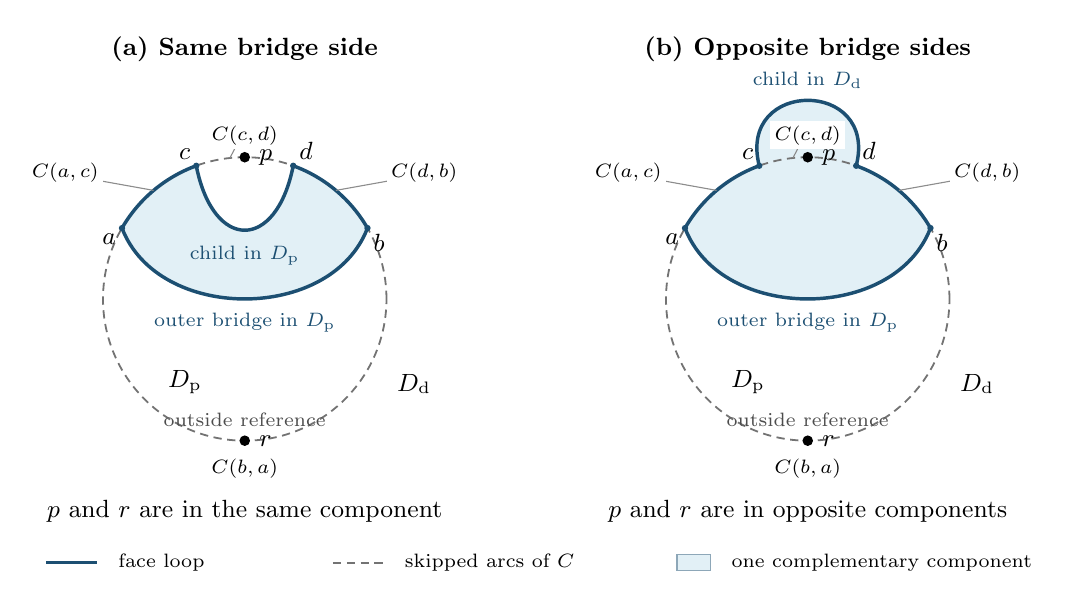
\begin{tikzpicture}[x=1cm,y=1cm,font=\small,
  tour/.style={draw=black!55,densely dashed,line width=.65pt},
  route/.style={draw=loopsideroute,line width=1.25pt},
  arcname/.style={font=\scriptsize,fill=white,inner sep=1.5pt},
  bridge/.style={font=\scriptsize,text=loopsideroute,inner sep=1pt},
  leader/.style={draw=black!45,line width=.4pt},
  testpoint/.style={circle,fill=black,inner sep=1.35pt}]

  \foreach \shift/\case in {0/0,7.15/1}{
    \begin{scope}[xshift=\shift cm]
      \coordinate (a) at (150:1.8);
      \coordinate (c) at (110:1.8);
      \coordinate (d) at (70:1.8);
      \coordinate (b) at (30:1.8);

      \ifnum\case=0
        \path[fill=loopsidefill]
          (a) arc[start angle=150,end angle=110,radius=1.8]
          .. controls (-.40,.60) and (.40,.60) .. (d)
          arc[start angle=70,end angle=30,radius=1.8]
          .. controls (1.10,-.30) and (-1.10,-.30) .. cycle;
      \else
        \path[fill=loopsidefill]
          (a) arc[start angle=150,end angle=110,radius=1.8]
          .. controls (-.90,2.80) and (.90,2.80) .. (d)
          arc[start angle=70,end angle=30,radius=1.8]
          .. controls (1.10,-.30) and (-1.10,-.30) .. cycle;
      \fi

      \draw[tour] (0,0) circle (1.8);
      \node at (-.76,-1.06) {$D_{\rm p}$};
      \node at (2.15,-1.08) {$D_{\rm d}$};

      \draw[route] (a)
        arc[start angle=150,end angle=110,radius=1.8];
      \draw[route] (d)
        arc[start angle=70,end angle=30,radius=1.8];
      \draw[route] (b)
        .. controls (1.10,-.30) and (-1.10,-.30) .. (a);
      \node[bridge] at (0,-.30) {outer bridge in $D_{\rm p}$};

      \ifnum\case=0
        \draw[route] (c)
          .. controls (-.40,.60) and (.40,.60) .. (d);
        \node[bridge] at (0,.55) {child in $D_{\rm p}$};
        \node[font=\small\bfseries] at (0,3.17)
          {(a) Same bridge side};
        \node[align=center,font=\small] at (0,-2.70)
          {$p$ and $r$ are in the same component};
      \else
        \draw[route] (c)
          .. controls (-.90,2.80) and (.90,2.80) .. (d);
        \node[bridge] at (0,2.78) {child in $D_{\rm d}$};
        \node[font=\small\bfseries] at (0,3.17)
          {(b) Opposite bridge sides};
        \node[align=center,font=\small] at (0,-2.70)
          {$p$ and $r$ are in opposite components};
      \fi

      \draw[leader] (-2.00,1.53) -- (130:1.8);
      \node[arcname] at (-2.28,1.60) {$C(a,c)$};
      \draw[leader] (2.00,1.53) -- (50:1.8);
      \node[arcname] at (2.28,1.60) {$C(d,b)$};
      \draw[leader] (-.10,1.96) -- (96:1.8);
      \node[arcname] at (0,2.08) {$C(c,d)$};
      \node[arcname] at (0,-2.16) {$C(b,a)$};

      \foreach \point/\place in {a/below left,c/above left,
                                  d/above right,b/below right}{
        \fill[loopsideroute] (\point) circle (1.15pt);
        \node[\place,inner sep=2pt] at (\point) {$\point$};
      }
      \node[testpoint,label={[inner sep=3pt]right:$p$}] at (0,1.8) {};
      \node[testpoint,label={[inner sep=3pt]right:$r$}] at (0,-1.8) {};
      \node[font=\scriptsize,text=black!70] at (0,-1.53)
        {outside reference};
    \end{scope}
  }

  \draw[route] (-2.52,-3.35) -- (-1.88,-3.35);
  \node[anchor=west,font=\scriptsize] at (-1.73,-3.35)
    {face loop};
  \draw[tour] (1.12,-3.35) -- (1.76,-3.35);
  \node[anchor=west,font=\scriptsize] at (1.91,-3.35)
    {skipped arcs of $C$};
  \path[fill=loopsidefill,draw=loopsideroute!50,line width=.4pt]
    (5.49,-3.45) rectangle (5.91,-3.25);
  \node[anchor=west,font=\scriptsize] at (6.06,-3.35)
    {one complementary component};
\end{tikzpicture}
\endgroup

\caption{The side test for an outer switch $[a,b]$ and its child
$[c,d]$.  The circle is the spatial resolved-tree tour $C$, separating
the primal and dual disks $D_{\rm p},D_{\rm d}$.  A point $p$ on
the skipped child arc lies with the exterior reference point $r$
exactly when both bridges use the same disk.  The bridge curves
represent narrow surgery strips in a topological drawing; their
lengths do not represent distances in the flag triangles.}
\label{loop:surgery-sides-figure}
\end{figure}

\begin{remark}\label{loop:count}
The finite drawing is a regular neighborhood of $(V(M_n),A_n)$.
If it has $k(A_n)$ components and $b_n$ boundary loops, its Euler
characteristic is both $|V(M_n)|-|A_n|$ and $2k(A_n)-b_n$.  Hence
$b_n=2k(A_n)+|A_n|-|V(M_n)|=\ell(M_n,A_n)$.  The surgery description
likewise gives one plus the number of flexible orders.  Thus the face
bijection counts the actual interfaces of the specified ensemble.
\end{remark}

\subsection{From chord convergence to complete loop matching}

Let $\mathcal L$ be the lamination underlying $\mathcal E$.  For a chord
with endpoints $a,b$, the peanosphere identification gives
$\eta(a)=\eta(b)$.  Thus there is a map
\[
 Q:\mathcal L\longrightarrow\Chat,
 \qquad Q(e^{2\pi it})=\eta(t),
 \qquad Q\big|_{[a,b]_{\rm d}}\equiv\eta(a).
\]
It is well defined and continuous.  To see continuity, consider a
convergent sequence of points on chords and extract convergent endpoint
pairs.  At a limit point in the open disk the limiting chord fixes the
value.  At a limit point of the time circle, strict convexity of the disk
forces that point to be an endpoint of the limiting chord, so the same
conclusion follows from $\eta(a)=\eta(b)$ and continuity of $\eta$.
For a face $F$ of $\mathcal L$, define $\ell_F$ to be the cyclic curve
$Q|_{\partial F}$.  Constant curves will be discarded.

We state the compactness argument in a form that also controls loops
whose indexing face varies with $n$.

\begin{lemma}[Convex cells and cyclic curves]\label{loop:convex}
In the common spatial correspondence the following assertions hold.
\begin{enumerate}
\item For every face $F$ of $\mathcal L$ and every $x\in F$, eventually
there is a unique face $F_n$ containing $x$, and
$\overline F_n\to\overline F$ in Hausdorff distance.  The associated
spatial FK loops converge to $\ell_F$ in uniform distance modulo cyclic
increasing reparameterization.
\item If $F_{n_j}$ is any sequence of faces, then after further extraction
$\overline F_{n_j}$ has a compact convex limit $K$.  If $K$ has interior,
it is the closure of one face of $\mathcal L$ and the corresponding
spatial loops converge cyclically to that face loop.  If $K$ has no
interior, the spatial loop diameters tend to zero.
\item The multiset of nonconstant $\ell_F$ is locally finite on the sphere.
For every $\varepsilon>0$, eventually there is a partial bijection between
the discrete and limiting face loops which covers every loop of spherical
diameter greater than $\varepsilon$, and each matched pair is at
individual-loop distance at most $\varepsilon$.
\end{enumerate}
\end{lemma}

\begin{proof}
Chord endpoint convergence implies Hausdorff convergence of the underlying
laminations.  A compact connected subset of $F$ has positive distance
from $\mathcal L$ and therefore lies in one discrete face eventually.
Exhausting $F$ by such compact subsets gives
$\overline F\subset\liminf\overline F_n$.  Every boundary chord of $F$
is approximated by discrete chords, and $F_n$ lies on the side of each
approximating chord selected by $x$.  The intersection of these closed
half-disks is $\overline F$.  This gives the reverse inclusion and proves
the first cell assertion.

For a varying sequence, compactness of the space of compact convex
subsets of $\overline{\mathbb D}$ gives a limit $K$.  If $K$ has interior,
no limiting chord can cut that interior: an approximating chord would
cut the corresponding discrete face.  Choose an interior point of $K$
outside the lamination.  The first part then identifies $K$ with a face
closure.  Such a point exists, since otherwise the lamination would
contain an open disk in $K$; a chord through that disk would again cut
$K$, which is impossible.

For the curve assertion in this case, parameterize $\partial F_n$ and
$\partial F$ by radial bearings from a fixed interior mark.  Their radial
functions converge uniformly.  Indeed an interior disk about the mark is
contained in all sufficiently large $F_n$, and convexity then bounds the
radial modulus uniformly; pointwise convergence follows from the cell
convergence.  These boundary parameterizations preserve cyclic order.
On exposed circle arcs, the spatial routes converge to $\eta$ uniformly.
On a chord side, Lemma~\ref{loop:surgery} confines the route to a matched
quadrangle, whose image diameter tends to zero.  Every subsequential
limit of such a route is therefore the common endpoint value of $Q$.
The compactness argument used above to prove continuity of $Q$ makes this
convergence uniform on the parameter circle.  Pauses inserted at chord
endpoints are harmless: continuous nondecreasing changes of time are
uniform limits of strictly increasing changes of time and give the same
zero-distance class in the stated loop topology.

Suppose instead that $K$ has no interior.  It is a point or a line
segment.  A closed convex cell is the convex hull of its contacts with
$\partial\mathbb D$.  Extracting those compact contact sets shows that
$K$ is the convex hull of its limiting circle contacts.  There are at most
two such contacts, since three distinct points of the circle are
noncollinear.  In the two-contact case, a boundary chord of a discrete
cell converges to their connecting segment.  For clarity, take a point
strictly between the two contacts and boundary points on either side of
it tending to the segment; these points are on chord sides, and any
limiting side through an interior point of the segment has exactly those
two circle endpoints.  The endpoints consequently have equal $Q$ values.
All exposed-circle route values and all chord-side route values have that
same subsequential limit.  Thus the spatial diameters tend to zero.

To prove local finiteness, suppose distinct limiting faces had loop
diameters bounded below.  Their closures have a subsequential convex
limit.  The preceding collapsed-cell argument, applied with the fixed
lamination, rules out an empty interior.  If the limit has interior, an
interior disk is eventually contained in every face in that subsequence,
contradicting disjointness of distinct faces.  Thus only finitely many
limiting face loops have diameter above any positive threshold.

Fix $\varepsilon>0$.  Match all limiting face loops of diameter greater
than $\varepsilon/2$ to the discrete faces selected by their interior
marks.  There are finitely many, their selected faces are distinct for
large $n$, and their cyclic errors tend to zero.  If unmatched discrete
loops of diameter greater than $\varepsilon$ remained along a subsequence,
Part~2 would produce a noncollapsed limiting face loop of diameter at
least $\varepsilon$.  Its interior mark would eventually belong to the
unmatched discrete face, contrary to the selected matching.  This proves
the final assertion, and a diagonal sequence of $\varepsilon$ gives the
claimed loop-ensemble topology.
\end{proof}

\subsection{The alternating exploration convention}

We now identify the limiting curves.  Put the exploration root at
$\infty$, and adjoin independent uniform times $U_1,U_2,\ldots$.
Their images $z_j=\eta(U_j)$ are area-typical targets.  Almost surely
these times are dense, the targets are dense in the sphere, and they
avoid all CLE loop traces.  We work on
one event on which the assertions below hold for all these targets and
all rationally truncated exploration windows.
Indeed the countable construction of the CLE loops and the frontiers
at rational times in a smooth spherical-area parameterization
are determined before the independent quantum field is sampled.
Their traces have zero Lebesgue area and consequently zero quantum
area almost surely.  A multiply visited point lies on such a frontier
between two of its visits.  Thus typical targets also have unique
visit times.

The exploration tree is the one determined by the imaginary field in
Section~\ref{local:section}.  Its branch toward $z_j$ is obtained from the
space-filling curve by erasing the fillings disconnected from $z_j$.
After a strict initial cut it is radial
$\mathrm{SLE}_{\kappa}(\kappa-6)$ in its target component.  The marked
boundary prime end and the growing tip have angular separation
$\theta\in[0,2\pi]$.  We use the following convention for extracting
\emph{nested} CLE from this tree: traverse a full excursion of $\theta$
from one endpoint of $[0,2\pi]$ to the other, complete its loop by the
branch aimed at the excursion's starting point, and repeat in the
remaining target component.  The completing branch approaches the
later prime-end lift of that point from the component separated from
the target at the end of the excursion.  This is the approach which
makes the starting point its terminal second visit
\cite[Section~2.1.6 and Figure~4]{AruHoldenPowellSunCritical}.
The directions alternate.  This precise
iteration is described in
\cite[Remark~2.3 and Sections~2.1.6--2.1.7]{AruHoldenPowellSunCritical}.
The whole-plane branching construction is that of
\cite[Section~2.3.1]{GwynneMillerQianCLE}; its whole-plane and local
radial laws are those of \cite[Section~2.1.3]{MillerSheffieldIGIV}.

\begin{lemma}[The unmarked law of the alternating construction]
\label{loop:ensemble-law}
The ensemble obtained by this alternating construction from the
whole-plane tree has the law of whole-plane $\mathrm{CLE}_{\kappa}$.
It is locally finite, its loops do not trace themselves or each other,
and its unmarked law is invariant under M\"obius transformations.
\end{lemma}

\begin{proof}
First consider a radial branching tree in a proper simply connected
domain $D$, with force point immediately on either side of its boundary
root.  The alternating construction is the nested-domain construction
of \cite[Section~2.1.6]{AruHoldenPowellSunCritical}.  Its first full
crossing, completed through the separated component, gives an outermost
loop.  The component of its complement containing a target is exactly
the radial target component at the crossing time.  Conditional on the
explored branches and completions, the unexplored trees in the
components are independent radial trees.  At the next generation the
force side is reversed, as follows from $\theta\mapsto2\pi-\theta$
and the strong Markov property
\cite[Remark~2.3]{AruHoldenPowellSunCritical}.  Reflection preserves the
unmarked domain CLE law.  Induction for finitely many targets and
generations, followed by the countable union, therefore gives the
independent-domain iteration defining nested $\mathrm{CLE}_{\kappa}$.
This also gives consistency at a discovered interior bubble: its
descendant loops are exactly those of the continued tree in that bubble,
and other loops of the domain ensemble cannot enter its interior.
Thus the two crossing directions give consecutive generations in this
construction.

We pass to the whole plane using stopping domains.  Choose a
deterministic target, put it at $0$, and use the bi-infinite Loewner
time of its branch from $\infty$.  Define
\[
 S_m=\inf\{t\ge -m:\theta(t)\in\{0,2\pi\}\},\qquad
 T_m=\inf\{t\ge S_m:\theta(t)=2\pi-\theta(S_m)\}.
\]
These are stopping times.  Full angular crossings occur arbitrarily
far toward the initial end
\cite[Lemma~2.7]{GwynneMillerQianCLE}, so $T_m\to-\infty$ almost
surely.  Explicitly, fix any earlier full crossing.  Once $-m$ precedes
its starting endpoint visit, $T_m$ is no later than its ending visit:
whichever endpoint is hit first after $-m$, both endpoints have been
visited by then.

Let $D_m$ be the component containing $0$ after $T_m$.  The tip and
force prime end coincide in the endpoint state $\theta(T_m)$.
The whole-plane strong Markov property and conditional
independence of branches after target separation imply that the
unexplored tree in $D_m$, conditionally on the exposed branch, is a
radial branching tree with the indicated endpoint force side
\cite[Proposition~2.2 and Section~2.1.3]{MillerSheffieldIGIV}.
The preceding domain argument shows that its future ensemble
$\Gamma^{(m)}$ has conditional law $\mathrm{CLE}_{\kappa}$ in $D_m$.
Its curves lie in $\overline D_m$ and may touch $\partial D_m$.

We check consistency with the global readout using only these domain
ensembles.  Fix a globally generated loop $G$ with target $w$ and a
finite starting crossing.  For sufficiently large $k$, the cut $T_k$
precedes both the separation of $w$ from $0$ and that crossing.  Then
$w\in D_k$, its branch shares the exposed prefix, and $G$ is a loop
of $\Gamma^{(k)}$: every subsequent full crossing and its completion
are computed from the same restricted tree.  Increase $k$ so that
$T_k<T_m$ as well.  In the domain construction for $\Gamma^{(k)}$,
$T_m$ is a later full-crossing time toward $0$, and $D_m$ is the
corresponding interior bubble.  Domain consistency therefore says
that $G$, if its trace enters $D_m$, is a descendant loop generated by
the continued tree there, hence belongs to $\Gamma^{(m)}$.
Conversely every loop of $\Gamma^{(m)}$ is a global crossing loop.
There are countably many cuts and generated loops, so these statements
hold simultaneously.  In particular the global and future readouts
agree on all loop tests in a compact subset of $D_m$, including loops
which touch $\partial D_m$ elsewhere.

The branch tends to $\infty$ at its initial end.  Thus every fixed disk
lies in $D_m$ eventually: for sufficiently negative $T_m$ the entire
exposed past lies outside that disk, whose connected interior belongs
to the $0$-component.  The domain limit theorem
\cite[Theorem~A.1]{MillerWatsonWilsonNestingField} identifies the limit
of $\mathrm{CLE}_{\kappa}$ in such domains with the unique whole-plane
law.  Its conformal matching estimate is uniform over all proper simply
connected domains, with error tending to zero as their boundary recedes
from a fixed disk.  It applies conditionally to $D_m$: bounded
continuous tests of the loop configurations in a fixed compact set
converge to the fixed whole-plane expectation, and dominated convergence
removes the conditioning.  The local agreement just proved identifies
the global alternating readout with this limit.  It also transfers
local finiteness and the absence of shared arcs directly from a domain
ensemble, since every compact set is eventually inside some $D_m$.

The whole-plane construction in \cite[Section~2.3.2]{GwynneMillerQianCLE}
uses a positive-crossing subsequence.  Its agreement in law with this
same large-domain limit is stated in Remark~2.6 of that paper.
Consequently its M\"obius-invariance theorem
\cite[Theorem~1.1]{GwynneMillerQianCLE} applies to the present unmarked
ensemble.
\end{proof}

We use no tracing in the strong sense of
\cite[Definitions~2.4--2.5]{GwynneMillerQianCLE}: no nonconstant
open portion of a traversal has its image contained in the union of
the complementary trace and the traces of finitely many other loops.  Reference
CLE traversals are parameterized without constant intervals; pauses
will be allowed when comparing them with face contours.  This
image-containment statement, rather than merely the absence of an
identical parameterized subarc, will be needed below.

The next dictionary relates three orders.  The interval $[a,b]$ uses
the quantum-area time of the space-filling curve: $a$ enters a filled
bubble and $b$ completes it.  Along a target branch, larger enclosing
intervals are encountered first.  Its moving clock erases the off-target
fillings while retaining the ordered branch trace.  The two endpoints
of a full angular crossing in branch time will be denoted by
$\sigma,\tau$; they need not be the area times $a,b$.

\begin{lemma}[Cone intervals and exploration switches]
\label{loop:switches}
For each typical target time $u$, the cone intervals containing $u$
describe the successively filled target bubbles.  Their order along the
branch toward $\eta(u)$ is reverse inclusion.  Their entrance-wall labels
are the two endpoint states of $\theta$, up to a fixed interchange.
Consequently a last closure of one type before a closure of the other
type starts the between-tips portion of a nested CLE loop.  The tree
completes that loop inside the larger interval's filling.

These switches recover all loops surrounding the target, once each.
Every typical target surrounded by such a completed loop belongs to its
outer interval's filling.  Enclosing cone intervals approach the full
time interval at the root end, and arbitrarily small such intervals
contain $u$.

For every fixed strict interior horizon, ancestor-free erasure has a
continuous moving trace.  In every nonempty interval of its moving
clock, erased intervals of both entrance-wall types occur.
\end{lemma}

\begin{proof}
We give the frontier dictionary in the cut surface, where different
prime ends over one spatial point remain distinct.  Color the left
side of the branch red and its right side blue.  The boundary of its
current target component consists, in prime-end order, of a red arc
and a blue arc between the tip $W$ and the marked junction $O$.
These are the boundary colors and exploration order of
\cite[Section~2.1.7 and Figure~9]{AruHoldenPowellSunCritical}.
The force prime end is precisely this junction $O$: it is transported
by the Loewner map until a collision, and the same boundary-color rule
continues it after the collision.  The two prime-end arcs have strictly
positive quantum length when they are nontrivial.  Therefore one color
is absent exactly when $O$ and $W$ coincide on the corresponding side,
that is, when $\theta=0$ or $\theta=2\pi$.

We use the precise bubble readout of
\cite[Section~2.3.4, Definition~2.2 and Figure~4; Lemma~3.1]
{GwynneMillerSLECharacterization}: a filled bubble has interval
$[v(b),b]$, its boundary length is $|Z(b)-Z(v(b))|$, and its side
is specified by the coordinate equal at the two endpoints.  This
statement uses backward cone intervals, with the same entrance
convention as here.  The following frontier verification explains
its use on the sphere.  When a
monocolored component is entered at time $a$, the space-filling order
visits all its descendants before returning to a different component;
write $b$ for its completion time.  Its interior is visited only during
this block, although its boundary points may be visited again.
The frontier outside this component
is unchanged throughout its filling.  Subtracting its terminal heights
therefore gives the two remaining frontier lengths
\begin{equation}\label{loop:frontier-lengths}
 \bigl(L(s)-L(b),\ R(s)-R(b)\bigr),\qquad a\le s\le b.
\end{equation}
They are nonnegative, both are zero at $b$, and exactly one is zero
at $a$.  The first entry $a$ is the entrance $v(b)$: in the
running-minimum frontier construction of
Theorem~\ref{enc:peanosphere}, extending the block farther backwards
crosses one of its two terminal frontier levels.

The converse uses the same frontier construction.  For a cone interval
$[v(b),b]$, cut the two frontier trees at heights $L(b)$ and $R(b)$
and retain its filling block.  The horizontal identifications inside
the block stay above those cuts.  Its unfilled boundary arcs are
parameterized by the height intervals in
\eqref{loop:frontier-lengths}; at its first time the arc for the
entrance wall is empty.  Maximality of $v(b)$ prevents a preceding
block from remaining on these same two sides of the cuts.  Thus this
is exactly the monocolored component entered there.  If the interval
contains $u$, it is the branch's target component, since its interior
contains $\eta(u)$; if it precedes $u$, it is an erased off-target
filling.  This verifies both directions of the readout without imposing
a new law on the field inside the component.  Erasing earlier
off-target fillings does not change these two boundary arcs in the
target component.  The argument concerns the restricted quotient and
its length coordinates on $[a,b]\Subset(0,1)$, which are the same
in the sphere realization of Theorem~\ref{enc:peanosphere}; no
infinite-volume surface law is being assigned to that block.

Combining \eqref{loop:frontier-lengths} with the prime-end description
identifies the entrance-wall labels with the two endpoint states of
$\theta$, up to interchanging the colors.  Target components shrink
along a branch, and their contiguous filling blocks are consequently
ordered by reverse inclusion.  The exact backward-cone erasure for a
target branch is also stated in
\cite[Section~4.2 and Definition~4.14]{AruHoldenPowellSunCritical};
the ancestor-free construction underlying it is
\cite[Proposition~1.13 and Lemma~10.4]{DMSMating}.

Starting at either state, the last visit to it before reaching the other
is the beginning of a full crossing of $[0,2\pi]$.  The alternating
constructor therefore gives precisely the stated switches and their
between-tips portions.  Conditional on that portion, the remaining
piece is chordal SLE in the specified prime-end component, as in
\cite[Section~2.1.6]{AruHoldenPowellSunCritical} and
\cite[Section~2.3.2]{GwynneMillerQianCLE}.  More precisely, let
$\sigma,\tau$ be the starting and ending branch times of the full
crossing, and view the target bubble at $\sigma$ in its prime-end disk.
The tip and force point coincide at its designated boundary root $x$.
The completing branch approaches the later lift of this same $x$
through the component separated from the target at $\tau$.  The
excursion and completion therefore give a closed continuous curve
$\beta$ in the closed prime-end disk, starting and ending at $x$.
Both pieces lie in the larger cone interval's filling.

Let $f$ map that disk to the outer bubble.  Its continuous extension
exists because the boundary is locally connected.  The closed curves
$f((1-\varepsilon)\beta)$ lie in the bubble and converge uniformly to
the completed loop as $\varepsilon\downarrow0$.  Simple connectedness
gives zero winding about every point outside the bubble for each
approximant.  Winding stability gives the same assertion for the
completed loop at every off-trace point outside the bubble.  Thus every
surrounded typical target is in that bubble.

Iteration supplies exactly the successive nested loops about a target.
Their domains decrease to that target.  In the whole-plane version they
also exhaust toward the initial point.  Equivalently, the full crossings
of the recurrent angular diffusion occur at all scales; the whole-plane
branch is transient at its initial end and tends to its target at its
terminal end.  For any fixed compact subinterval of $(0,1)$, large
enclosing bubbles contain its image.  Their fillings therefore contain
that time subinterval, and their endpoints tend to $0,1$.

Finally, for the unconditioned Brownian contour, the two boundary
processes after ancestor-free erasure, read in forward branch order,
have negative jumps and stable index
$\kappa/4\in(1,2)$, one for each side
\cite[Proposition~1.13]{DMSMating}.  This reverses the time direction
of the positive-jump processes in that statement.  Each L\'evy measure has
infinite mass near zero, so each coordinate has jumps in every nonempty
clock interval.  The jumps are precisely the erased cone intervals of
the indicated wall type.  The time-changed trace is continuous directly:
every inverse-clock jump skips an interval $[a,b]$ with
$\eta(a)=\eta(b)$, and $\eta$ is continuous.  This is the inverse-clock
argument in \cite[Proposition~10.6]{DMSMating}.
The erasure retains the full ordered branch traversal; the skipped
intervals are space-filling visits to off-target bubbles, not moving
pieces of that branch.  Thus a portion on which the branch changes
position occupies a nonempty interval of its moving clock.
For the excursion, exhaust by strict interior rational windows
containing the full Brownian-time span of the tested clock interval,
including all its erased intervals.  Local absolute continuity
transfers the null event that one label is missing there.  Taking the
countable intersection gives the assertion for rational and independent
uniform horizons.  Only this almost-sure property is transferred;
the excursion's time-changed coordinates need not be L\'evy processes.
\end{proof}

\subsection{Ordered prefixes of the limiting face curves}

We now return to the cyclic curves supplied by
Lemma~\ref{loop:convex}.  The exploration dictionary will identify
successively longer prefixes of each such curve with one CLE
traversal.  First, contour genericity makes the order of a parent
and its child unambiguous.

\begin{lemma}[Strict endpoints of nested cone intervals]
\label{loop:strict-endpoints}
If two nondegenerate cone intervals in $(0,1)$ are distinct and one
contains the other, then both containments of their endpoints are strict.
\end{lemma}

\begin{proof}
Two intervals with the same terminal time have the same entrance
$v(t)$, so are equal.  Suppose instead that $[a,d]$ is properly
contained in $[a,b]$ and has the same entrance.  Interchange the two
coordinates if necessary so that the outer wall is $R$:
$R(a)=R(b)$ and $R\ge R(b)$ on $[a,b]$.
If the inner wall is $L$, its cone inequality and the outer inequality
give $R(a)\ge R(d)\ge R(b)=R(a)$.  Hence $[a,d]$ is both an
$L$-chord and an $R$-chord, contrary to
Lemma~\ref{enc:chord-genericity}(i).
If the inner wall is also $R$, then
$R(a)=R(d)=R(b)$, and $d$ is a scalar local minimum at that level,
strict by Brownian scalar genericity.
But $b$ is a backward joint record with positive witness, so its
$R$-height cannot be a scalar branch level by
Lemma~\ref{enc:chord-genericity}(ii).  This rules out a shared entrance
as well.
\end{proof}

The \emph{outer chord} of a face means its boundary chord which separates
it from the time-circle point $0$.  If its interval is $[a,b]$, its
\emph{children} are the other boundary chords, with intervals inside
$(a,b)$.  They are the maximal proper cone intervals skipped by that
face.  Write $K_F=\partial F\cap\partial\mathbb D$ for its circle
contacts, read in increasing time from $a$ to $b$.  Extending
$\eta|_{K_F}$ constantly across each child interval gives the ordered
face contour $\alpha_F:[a,b]\to\Chat$.  Its two endpoint values agree.

\begin{lemma}[Ordered prefixes from children]\label{loop:prefixes}
Every face with interior has an outer chord with endpoints in $(0,1)$.
If an immediate child has the opposite label, the portion of
$\alpha_F$ from $a$ to that child's entrance is a nonconstant initial
portion of the CLE loop indexed by their switch.

Every switch toward a typical target has exactly one incident face
with this prefix.  For every nonconstant face contour there is a
sequence of opposite-type children whose identified prefixes extend
one another and whose remaining contour diameters tend to zero.
In particular, $\alpha_F$ is a closed initial portion of one oriented
CLE traversal, up to pauses.
\end{lemma}

\begin{proof}
The enclosing chords of Lemma~\ref{loop:switches} approach the full
time interval.  An interior point of a face eventually lies between
one of those chords and the opposite circle arc.  The maximal circle
gap of that face containing time $0$ therefore has endpoints in
$(0,1)$.  Its bounding chord is the asserted outer chord.  Almost every
time in $(a,b)$ is inside a child: typical times have arbitrarily small
enclosing cone intervals, whereas no cone chord can cut the interior
of $F$.  We henceforth impose this fact for the independent uniform
targets as well as for almost every time.

Let $[c,d]$ be a child and take a target horizon $r\in(c,d)$.
Ancestor-free erasure toward $r$, restricted to $[a,c]$, is exactly the
face contour.  Here is the elementary nesting check.  Every child
interval before $c$ is a filling disconnected from that target and is
erased.  Conversely a deleted cone interval meeting a retained circle
contact would have to cross the outer chord or a child chord, unless
it were contained in one of the skipped children.  Crossing is
impossible, and the latter case deletes no further face contact.
Endpoint differences are constant pauses.  Thus the two procedures
retain the same points in the same order.

For an opposite-type child, there is no intermediate containing
interval between it and $[a,b]$, by maximality of the child.
Lemma~\ref{loop:strict-endpoints} gives $a<c<d<b$.  Their
closures are consequently the two endpoints of a full-winding
excursion in Lemma~\ref{loop:switches}.  The preceding erasure check
identifies the face prefix with its between-tips branch segment.  That
segment is nonconstant: a full crossing of the angular interval makes
a nontrivial Loewner hull.  Its traversal order is the branch order.

Conversely, take the two consecutive nested intervals of a target
switch.  A chord from the target time on the circle to time $0$,
outside the larger interval, crosses both bounding chords.  The open
segment between those crossings meets no lamination chord.  A chord
meeting it would separate these two circle points and therefore give
an intermediate interval containing the target.  The endpoints of the
segment are distinct, since the two bounding chords are distinct and
their intersections are in their relative interiors.  Closedness of
the lamination puts this open segment in one complementary face.
That face has the two specified chords on its boundary.  This proves
existence; the side of the outer chord fixes uniqueness.  It also
proves that the face has interior even when chords accumulate on
either side of the branch.

We next make the exhaustion assertion precise.  On a varying compact
subarc of $\alpha_F$ before a later varying portion, choose a child
strictly after it and a rational horizon inside that child.  Such a
child exists because almost every intervening time is in a child,
and a child cannot skip two retained contacts with distinct images.
The preceding erasure check identifies the earlier subarc with an
interval of this horizon's ancestor-free trace.  By
Lemma~\ref{loop:switches}, this is the full ordered moving trace.
Its portion between distinct spatial values therefore occupies a
nonempty interval of the moving clock: an interval collapsed by that
clock is a skipped filling whose two endpoint images agree.
On this compact earlier part of the trace, the erasure check identifies
its retained set with the face contacts, up to endpoint pauses.  The
jumps of the inverse clock are the maximal open gaps of this retained
set, hence precisely the immediate child intervals there.  An interval
inside an already skipped child is not another inverse-clock jump.
The compact restriction before the later child's entrance removes any
cutoff at the target horizon.  The last assertion of
Lemma~\ref{loop:switches} therefore gives immediate children of both
labels on the chosen varying portion.  This use of the stable processes is simultaneous
for all rational horizons and all interior windows; the face and
subarc may therefore be chosen afterwards.

Set $x_0=\alpha_F(b)$.  Given a sufficiently small $\delta>0$, let
$t_\delta$ be the last time with
$\rho(\alpha_F(t_\delta),x_0)\ge\delta$.  There is a varying portion
after $t_\delta$ and before the contour becomes constant at $x_0$.
Apply the preceding paragraph to a compact part of that variation,
leaving some variation after it.  An opposite-type child entrance
$c_\delta>t_\delta$ occurs there, and
\[
 \diam_\rho\alpha_F([c_\delta,b])\le2\delta.
\]
Choosing successively smaller $\delta$ and later varying subarcs
makes the entrances nondecreasing.  If a constant terminal interval
is present, the entrances approach its first point and the same bound
holds.  This produces nested nonconstant prefixes with vanishing
remaining diameter.

All these prefixes belong to the same CLE loop: each contains the
first nonconstant prefix, and distinct CLE loops share no nonconstant
arc.  They also follow the same oriented traversal from the same
starting prime end.  No self-tracing prevents switching to a different
visit of that initial arc.  Parameterize this traversal on $[0,1]$;
the prefix endpoints are nondecreasing parameters, bounded by $1$,
and hence converge to a parameter $s$.  Continuity of that traversal
and the vanishing remainder diameter identify the face contour with
the traversal up to $s$, allowing pauses.  Since the face contour is
closed, it is a closed initial portion, as asserted.
\end{proof}

\subsection{A winding test for an omitted strand}

The prefix lemma leaves a specific possibility: a face contour might
close before its CLE traversal has finished.  Equality of traces would
not settle this question of order.  We instead show that any omitted
moving portion changes winding around an open set, which the finite
side test can detect.

For an oriented closed curve $A$ and a point $z$ outside its trace,
$\operatorname{Ind}(A,z)$ denotes its integer winding number.  We use
the orientation inherited from the exploration; a CLE loop has index
zero or its designated sign.  In particular its nonzero-index components
are exactly its surrounded components.  No rectifiability is needed:
the index is the degree of the map from the parameter circle to the
unit circle viewed from $z$.

\begin{lemma}[An omitted moving portion changes a winding test]
\label{loop:strand}
Almost surely, simultaneously for every loop $L$ of the exploration
ensemble, the following holds.  Let $P$ be a closed initial portion of
its oriented traversal.  If the omitted portion is nonconstant, there
is an open disk $V$ disjoint from the trace of $L$ such that
\[
 \operatorname{Ind}(P,z)\ne\operatorname{Ind}(L,z),\qquad z\in V.
\]
Consequently equality of these indices on a dense off-loop target set
forces $P$ to be the whole traversal, up to pauses.
\end{lemma}

\begin{proof}
The deterministic step is a local index comparison.  Suppose that a
closed curve $C$ and $L$ share an oriented compact segment $A$, and
write $L=A*B$, $C=A*E$.  If the complementary arcs $B,E$ miss a
connected ball $U$, then additivity of degree gives
\begin{equation}\label{loop:index-difference}
 \operatorname{Ind}(L,z)-\operatorname{Ind}(C,z)
   =\operatorname{Ind}(B*\overleftarrow E,z),
 \qquad z\in U\setminus L.
\end{equation}
The right side is constant on $U$.  Consequently, if two off-trace
points of $U$ have different indices for $C$, they also have different
indices for $L$.  If $P$ misses $U$, its index is constant there and
cannot agree with $L$ at both points.  Local constancy off compact
traces then gives the disk $V$ in the statement.

We will apply this comparison with $C$ a chordal SLE closed along a
boundary side.  To cover an initial portion chosen after seeing the
loop, we first construct one simultaneous family of comparison paths.
Every moving open portion of a loop contains an interior segment with
law absolutely continuous with respect to a segment of ordinary
chordal $\mathrm{SLE}_{\kappa}$.  Indeed each loop is its full-winding
branch piece followed by its conditional chordal completion.  In the
first piece use countably many windows stopped while the driving and
force points are separated by at least $1/m$, in a fixed bounded time
window after a strict initial cut.  The force drift is bounded there,
and coordinate change followed by Girsanov gives the asserted local
absolute continuity \cite[Theorem~3 and Section~5]
{SchrammWilsonCoordinateChanges}.  Force collisions have no time
interval.  In the completion use its conditional chordal law in the
cut domain.  Each moving interval contains an interior excursion:
a continuous Loewner trace spends zero capacity time on the domain
boundary \cite[Proposition~1.7]{YuanLoewnerTraces}.  Restrict to a
compact subinterval of such an excursion.  Enumerate the countably many
branches, completions, and stopped windows, and refine them by all
rational compact subintervals in these interior excursions.  The
resulting countable family of comparison segments contains a member
inside every moving open portion, including those selected subsequently.

An ordinary chordal SLE in a Jordan disk has open pockets of both
passage sides arbitrarily close to each moving interior trace point.
To verify the needed two-sided assertion, decorate a quantum wedge by
an independent chordal SLE.  Its left and right boundary-length
processes in quantum natural time are independent spectrally negative
stable processes of index $\kappa/4$
\cite[Theorem~10.1]{DMSMating}.  Both have jumps in every nonempty time
interval, and each jump cuts off an open pocket on its designated side.
We need this clock to describe the full ordered traversal, as well
as to be continuous.  The proof of \cite[Theorem~1.16]{DMSMating},
with both force weights zero, obtains ordinary chordal SLE by welding
two wedges of weight $\gamma^2-2$ to a middle wedge of weight
$2-\gamma^2/2$; the ambient weight is $3\gamma^2/2-2$.
In the middle wedge the interface is a concatenation of
$\mathrm{SLE}_{\kappa}(\kappa/2-4;\kappa/2-4)$ traces.
\Citet[Lemma~10.4 and Proposition~10.6]{DMSMating} identify its entire
ordered counterflow traversal and its continuous quantum-natural
parameterization.  The inverse-clock jumps skip space-filling visits
to bubbles, not moving portions of that counterflow traversal.

The exterior welding in the proof of Theorem~1.16 retains this same
interface and the ordered quantum bubbles it encloses.  The intrinsic
bubble description of quantum natural time in
\cite[Theorem~6.22, Definition~6.23 and Remark~10.5]{DMSMating}
therefore retains its clock, with the fixed deterministic normalization.
This construction gives a continuous parameterization of the full
ordinary chordal traversal.  Every moving portion thus occupies a
positive clock interval.  Jumps of each stable coordinate in every
rational clock interval, together with continuity, imply that closing
tips of pockets of both sides approach every moving interior trace
point simultaneously.  Interior points of these pockets may be chosen
arbitrarily close to their tips and remain off the entire chordal
trace.  These nearby interior points supply the two-sided test.
Integrating out the auxiliary field
gives the property for the unclocked chordal law.

Close the reference chordal path by one specified boundary side of the
disk.  Its winding indices on pockets of the two passage sides differ
by one.  One way to see this without a smoothness assumption is ordered
approximation of a continuous Loewner trace by simple traces
\cite[Theorem~1.1]{YuanLoewnerTraces}.  Truncate away from its terminal
point, complete within a shrinking terminal neighborhood, and close
on the same boundary side.  The Jordan curve theorem gives the side
test for each approximant, and uniform convergence preserves winding
about any fixed off-trace points.  For a cut domain perform this argument
in its prime-end disk, using only interior test points.  Hence the
assertion survives conformal coordinates and the stopped local changes
of measure above.

The full ordinary chordal reference law also has strong no self-tracing.
For a fixed indexed full crossing, the conditional completion given
the explored trunk is ordinary chordal SLE in its remaining component,
and its concatenation with the trunk is a CLE loop
\cite[Section~2.3.2]{GwynneMillerQianCLE}.
Normalize this component to a prime-end disk.  An open portion whose
image there lay in its complementary trace would give the same
containment in the physical CLE loop.  It has an interior moving
subinterval by \cite[Proposition~1.7]{YuanLoewnerTraces}; conformal
injectivity there prevents its physical image from being constant.
This contradicts the strong CLE property stated above.  The normalized
completion has the fixed ordinary chordal law conditionally on the
trunk, so the deduction gives a probability-one property of that law.
The same interior argument transfers it to the cut-domain reference
paths used here.

Before choosing any initial portion, retain a complete reference path
for every member of the countable comparison family.  For one member,
disintegrate its reference chordal law given the compared segment and
weight by the Radon--Nikodym derivative of the actual segment law.
Sampling from this conditional extension kernel couples the actual
segment with a complete chordal path which agrees with it; the full
path marginal is absolutely continuous with respect to chordal SLE.
These kernels exist on the continuous-path spaces.  Use auxiliary
randomness for the countably many extensions, and intersect all their
no-tracing and two-sided-pocket events, together with the corresponding
events for the original loops.  This gives a single probability-one
event on the enlarged space.

On that event fix arbitrary $L$ and $P$.  The omitted moving portion
cannot have its entire trace in $P$, by no self-tracing.  It therefore
contains a moving open interval whose trace misses the compact trace
of $P$.  Choose an already enumerated comparison segment inside it,
and let $c$ be its already retained complete reference path.  Thus $c$
and $L$ agree on an open parameter segment, and the required properties
of both full curves hold before this choice.

For any continuous curve with no self-tracing, the set of repeated
parameter times is meagre.  To check this, for disjoint compact rational
parameter intervals $J,K$, the set of times in $J$ whose images lie in
the image of $K$ is closed.  It has empty relative interior: otherwise
an open portion would have its image contained in the complementary trace, violating
the strong no-tracing property.  The countable union of
these sets covers all repeated times, with the cyclic endpoint
convention for $L$.  Apply this to both $L$ and the complete path $c$.
On their common open segment choose, by the Baire theorem, a time
visited only once by each full curve.  Let its position be $x$.

Choose a smaller common compact segment $A$ around that time.  Both
complementary arcs are compact and miss $x$.  There is consequently a
ball $U$ about $x$ which misses these two complementary arcs, $P$, and
the cut-domain boundary.  Close $c$ by its boundary-side arc to obtain
$C$.  Inside $U$, the only portions of $L$ and $C$ are their identical
oriented segment $A$.  The two passage pockets of $c$ supply points
of $U$ at which the indices of $C$ differ by one.  The deterministic
comparison \eqref{loop:index-difference} now supplies the required
open disk $V$.

All subsequent choices are deterministic on the single event just
constructed.  The conclusion therefore holds for every closed initial
portion.  Since this conclusion concerns only the original loops,
integrating out the auxiliary reference paths gives the asserted
probability-one event on the original space.
\end{proof}

\subsection{Identification with all nested CLE loops}

\begin{theorem}[Complete CLE readout]\label{loop:readout}
The nonconstant curves $\ell_F$, with their cyclic orders and with
orientations forgotten, are exactly the whole-plane nested
$\mathrm{CLE}_{\kappa}$ ensemble determined by the independent
space-filling exploration.  Each CLE loop occurs once.
\end{theorem}

\begin{proof}
We first transfer the finite side test to a fixed face.  For each fixed
boundary chord of $F$, the corresponding sides of its approximating
faces have the same limiting endpoints.  To verify this, take a point
in the relative interior of that chord and a transverse line through
it meeting $F$.  The endpoints of the resulting convex-cell sections
converge.  Their supporting chord sides have subsequential endpoint
limits on the circle; a limiting side through the chosen interior
point must be the full bounding chord, since its line has only two
circle intersections.  Lemma~\ref{loop:chords} then gives eventual
agreement of their labels.

Fix a typical target in one child and a test time outside the outer
interval, using time $0$ as the reference point at infinity.  These
locations are off the limiting face contour: by
Lemma~\ref{loop:prefixes}, that contour is an initial portion of a CLE
loop, and the targets avoid all CLE traces.  For a target time $u$
strictly inside a child, choose discrete tour times $u_n\to u$.
Convergence of the two child endpoints puts $u_n$ inside the
corresponding discrete child for all large $n$, and the spatial
correspondence sends its tour point to $\eta(u)$ in the limit.
The analogous assertion holds for the exterior reference point.
Their positive distance from the compact limiting contour and uniform
loop convergence preserve the finite winding test.
Lemma~\ref{loop:surgery} therefore implies
\begin{equation}\label{loop:side-test}
 \operatorname{Ind}(\alpha_F,\eta(u))\ne0
 \quad\Longleftrightarrow\quad
 u\text{ is in an opposite-type child of }F.
\end{equation}
Targets outside the outer interval have index zero.  The nonzero
index has the orientation sign of the prefix.  The statement holds
simultaneously for all faces and all the countably many targets;
there are only countably many faces, since each contains a rational
disk point.

By Lemma~\ref{loop:prefixes}, a nonconstant face is a closed initial
portion $P$ of one CLE loop $L$.  Conversely every CLE loop has a
surrounded open component, hence contains a typical target.  Its
switch supplies a face with a nonconstant prefix, so no CLE loop is
absent from this assignment.

We show that targets surrounded by one fixed $L$ give the same outer
interval.  Let $I_1,I_2$ be their switch outer intervals.  Every typical
target surrounded by $L$ lies in each outer bubble by
Lemma~\ref{loop:switches}.  Typical points have unique visit times,
so both intervals contain both target times and are nested.  Suppose,
for contradiction, that $I_2$ is a proper subinterval of $I_1$.
Let $J_1$ be the child of $I_1$ used by its switch.  The first target
time lies in the interiors of both $J_1$ and $I_2$.  These two
intervals are therefore comparable, and maximality of $J_1$ among
proper subintervals of $I_1$ gives $I_2\subseteq J_1$.  Thus the
second target also sees the switch
with outer interval $I_1$.  The between-tips prefix is identical for
both targets in that child, by target invariance and the erasure
description.  It identifies $L$ for both targets, since it is a
nonconstant shared arc.  But the second target already sees the
switch with outer interval $I_2$ producing $L$, contradicting the
once-only nested construction.  Hence $I_1=I_2$.  The face on its
inner side is unique, so every target surrounded by $L$ is tested
by an opposite-type child of the same face.

It follows from \eqref{loop:side-test} that $P$ and $L$ have the
same index on every typical target surrounded by $L$.  They also
agree on every typical target outside $L$.  Indeed targets outside
the outer interval have index zero.  A target inside it is almost
surely in a child; if it were in an opposite-type child, that switch
would produce a loop surrounding the target and sharing the
nonconstant prefix of $L$.  It would therefore be $L$, a
contradiction.  A same-type child has index zero by the side test.
The indices of $P$ and $L$ thus agree on the entire dense typical
target set.  Lemma~\ref{loop:strand} excludes any nonconstant omitted
portion.  Hence the face traverses the complete loop in its order.

Finally, two nonconstant faces assigned to the same $L$ would, by
their opposite-type children, supply two outer intervals for targets
surrounded by $L$.  We just proved that these intervals coincide;
their unique inner face is then the same.  This proves multiplicity
one and completes the identification.
\end{proof}

\begin{corollary}[Joint matching in the reference sphere]
\label{loop:matching}
On every common contour extraction, the collections $H_n(\widehat\Gamma_n)$
converge to the complete nested ensemble $\Gamma$ of
Theorem~\ref{loop:readout}, in the loop topology of the theorem.
The convergence is joint with the surface, area, and all additional
observations retained in the common extraction.  Every macroscopic loop on either
side is included in the matchings.
\end{corollary}

\begin{proof}
Combine Lemmas~\ref{loop:chords} and~\ref{loop:convex} with
Theorem~\ref{loop:readout}.  The topological correspondence is the
one of Theorem~\ref{top:homeomorphism}.  All limiting chord and face
data are measurable functions of the retained excursion, so the
identification holds in its existing joint coupling.  In particular,
it is not necessary to recouple an individual loop separately from
the other observations.
\end{proof}

\begin{proposition}[Canonical coordinates and independence]
\label{loop:canonical}
Before three-mark normalization, conditional on the reference quantum
surface, $\Gamma$ has the fixed unmarked whole-plane
$\mathrm{CLE}_{\kappa}$ law.  Let $T$ be the M\"obius map taking
three fresh independent quantum-area marks to $0,1,\infty$.
Then $T\Gamma$ has that same conditional law given the normalized
embedded quantum sphere.

On an extraction for which $\phi_n\circ H_n^{-1}\to f$ uniformly,
the canonical loop collections $\Gamma_n=\phi_n(\widehat\Gamma_n)$ converge to
$f\Gamma$.  Here $f=T$ or $f=\mathfrak r\circ T$, where
$\mathfrak r(z)=\overline z$; this is the same orientation alternative as
for all other retained observations.
\end{proposition}

\begin{proof}
The reference surface is decorated by an independent unclocked
space-filling SLE in Theorem~\ref{enc:peanosphere}.  Its exploration
tree and unmarked CLE are functions of that unclocked curve;
changing to the quantum-area clock changes neither.  Thus the
conditional loop law is fixed.  Given the surface and three fresh
area marks, $T$ is deterministic and the loop law remains unchanged
by its action: whole-plane $\mathrm{CLE}_{\kappa}$ is invariant
under every M\"obius transformation
\cite[Theorem~1.1]{GwynneMillerQianCLE}.  Taking conditional expectations and
then forgetting the unnormalized surface and marks proves the
claimed conditional independence in the normalized embedding.

For the convergence assertion, a uniform individual-loop matching
of error $\delta$ becomes a matching of error at most
\[
 2\|\phi_n\circ H_n^{-1}-f\|_\infty+\omega_f(\delta),
\]
where $\omega_f$ is a modulus of continuity of $f$ on the compact
sphere.  Uniform continuity of $f^{-1}$ ensures that every loop
of prescribed positive diameter in the new coordinate had diameter
bounded below in the old one.  Hence the complete matchings of
Corollary~\ref{loop:matching} remain complete after this coordinate
change.  Theorem~\ref{conf:canonical} identifies $f$ and its single
orientation sign, proving the last assertion.
\end{proof}
